\section{Experiments}
\label{sec:experiments}

\subsection{Experimental Setup} 

% \begin{figure*}[t]
%     \centering
%     \includegraphics[width=1\linewidth]{figs/5.pdf}
%     \caption{\textbf{Comparison of Token Cost and Accuracy Between GD and MAD under Different Agents and Rounds.} The notation (5,4) signifies 5 agents with 4 rounds. The results are average.}
%     \label{fig5}
%     % \vspace{-0.5cm}
% \end{figure*}

\begin{table*}[t]
\centering
\setlength\tabcolsep{1.5 pt}
\resizebox{\textwidth}{!}{
\begin{tabular}{ccccccccccc} 
\toprule
\multirow{2}{*}{Methods} & \multicolumn{2}{c}{GPQA} & \multicolumn{2}{c}{GSM8k} & \multicolumn{2}{c}{Arithmetic} & \multicolumn{2}{c}{MMLU} & \multicolumn{2}{c}{Math}  \\ 
\cmidrule{2-11}
& ACC(\%)$\uparrow$  & Tokens($k$)$\downarrow$   & ACC(\%)$\uparrow$   & Tokens($k$)$\downarrow$   & ACC(\%)$\uparrow$   & Tokens($k$)$\downarrow$       & ACC(\%)$\uparrow$    & Tokens($k$)$\downarrow$      & ACC(\%)$\uparrow$   & Tokens($k$)$\downarrow$    \\ 
\midrule
% \rowcolor{lightgray}
\rowcolor{Gray}
\multicolumn{11}{c}{\texttt{GPT-3.5-turbo-0125}} 
\\
\midrule
CoT                      & 31.2\scriptsize{$\pm 0.03$}  & 2.0\scriptsize{$\pm 0.02$}             & 76.8\scriptsize{$\pm 0.02$} & 0.25\scriptsize{$\pm 0.00$}         & 82.2\scriptsize{$\pm 0.04$} & 0.16\scriptsize{$\pm 0.02$}                & 70.2\scriptsize{$\pm 0.02$}  & 0.24\scriptsize{$\pm 0.00$}         & 35.2\scriptsize{$\pm 0.02$} & 0.37\scriptsize{$\pm 0.01$}           \\
CoT-SC(40)               & 31.2\scriptsize{$\pm 0.02$} & 80.5\scriptsize{$\pm 0.26$}          & \underline{\textbf{83.6}}\scriptsize{$\pm 0.01$} & \underline{10.0}\scriptsize{$\pm 0.02$}        & 95.0\scriptsize{$\pm 0.01$}  & 6.3\scriptsize{$\pm 0.11$}                 & \underline{\textbf{75.1}}\scriptsize{$\pm 0.02$}  & \underline{\textbf{9.6}}\scriptsize{$\pm 0.03$}         & \textbf{48.2}\scriptsize{$\pm 0.01$} & 14.6\scriptsize{$\pm 0.15$}           \\
MAD(5,3)                 & 31.2\scriptsize{$\pm 0.05$} & 42.7\scriptsize{$\pm 0.79$}          & 82.0\scriptsize{$\pm 0.01$}  & 13.7\scriptsize{$\pm 0.15$}        & 94.4\scriptsize{$\pm 0.01$} & 12.1\scriptsize{$\pm 0.27$}                & 68.8\scriptsize{$\pm 0.01$} & 16.0\scriptsize{$\pm 0.10$}         & 39.0\scriptsize{$\pm 0.02$}  & 16.5\scriptsize{$\pm 0.23$}           \\ 
GD(5,3)                  & \underline{\textbf{32.6}}\scriptsize{$\pm 0.05$} & \underline{36.9}\scriptsize{$\pm 0.46$}          & 81.6\scriptsize{$\pm 0.01$} & 10.3\scriptsize{$\pm 0.05$}         & \textbf{99.6}\scriptsize{$\pm 0.00$} & 9.6\scriptsize{$\pm 0.06$}                & 74.9\scriptsize{$\pm 0.03$} & 11.1\scriptsize{$\pm 0.07$}         & 37.8\scriptsize{$\pm 0.00$} & 13.7\scriptsize{$\pm 0.10$}           \\ 
\midrule
% \rowcolor{lightgray}
\rowcolor{Gray}
\multicolumn{11}{c}{\texttt{GPT-4-0613}} 
\\
\midrule
CoT                      & 50.2\scriptsize{$\pm 0.02$} & 2.0\scriptsize{$\pm 0.01$}           & 88.8\scriptsize{$\pm 0.01$} & 0.25\scriptsize{$\pm 0.00$}         & 94.4\scriptsize{$\pm 0.02$} & 0.20\scriptsize{$\pm 0.00$}                & 75.1\scriptsize{$\pm 0.02$}  & 0.28\scriptsize{$\pm 0.00$}         & 46.4\scriptsize{$\pm 0.05$} & 0.39\scriptsize{$\pm 0.01$}           \\
CoT-SC(40)               & 47.6\scriptsize{$\pm 0.02$} & 80.8\scriptsize{$\pm 0.18$}          & \underline{\textbf{91.0}}\scriptsize{$\pm 0.00$}  & \underline{10.0}\scriptsize{$\pm 0.01$}         & \underline{\textbf{100.0}}\scriptsize{$\pm 0.00$}     & \underline{8.3}\scriptsize{$\pm 0.03$}                & 78.8\scriptsize{$\pm 0.02$} & 5.7\scriptsize{$\pm 0.08$}         & \textbf{62.8}\scriptsize{$\pm 0.00$} & 15.3\scriptsize{$\pm 0.12$}           \\
MAD(5,3)                 & 48.4\scriptsize{$\pm 0.02$} & 46.1\scriptsize{$\pm 2.07$}          & 89.4\scriptsize{$\pm 0.00$} & 17.1\scriptsize{$\pm 0.06$}        & 98.4\scriptsize{$\pm 0.01$} & 12.5\scriptsize{$\pm 0.01$}                & 79.0\scriptsize{$\pm 0.02$} & 20.0\scriptsize{$\pm 0.11$}         & 56.2\scriptsize{$\pm 0.02$} & 22.3\scriptsize{$\pm 0.24$}           \\ 
GD(5,3)                  & \underline{\textbf{51.4}}\scriptsize{$\pm 0.03$} & \underline{36.9}\scriptsize{$\pm 1.11$}           & 89.8\scriptsize{$\pm 0.02$} & 11.0\scriptsize{$\pm 0.01$}         & 99.4\scriptsize{$\pm 0.01$} & 10.1\scriptsize{$\pm 0.33$}                & \textbf{83.7}\scriptsize{$\pm 0.01$} & 13.0\scriptsize{$\pm 0.12$}         & 57.2\scriptsize{$\pm 0.03$} & 15.1\scriptsize $\pm 0.19$ \\
\midrule
% \rowcolor{lightgray}
\rowcolor{Gray}
\multicolumn{11}{c}{\texttt{DeepSeek-R1-Distill-Qwen-32B}} 
\\
\midrule
CoT                      & 30.3\scriptsize{$\pm 0.02$} & 3.27\scriptsize{$\pm 0.57$}           & 90.7\scriptsize{$\pm 0.02$} & 0.58\scriptsize{$\pm 0.00$}         & 99.0\scriptsize{$\pm 0.01$} & 0.55\scriptsize{$\pm 0.00$}                & 79.9\scriptsize{$\pm 0.01$}  & 0.90\scriptsize{$\pm 0.02$}         & 56.3\scriptsize{$\pm 0.03$} & 1.62\scriptsize{$\pm 0.02$}           \\
CoT-SC(40)               & 57.7 \scriptsize{$\pm 0.02$} & 143.1 \scriptsize{$\pm 1.51$}          & 92.7\scriptsize{$\pm 0.00$}  & \underline{23.6}\scriptsize{$\pm 0.12$}         & \underline{\textbf{100}}\scriptsize{$\pm 0.00$}     & \underline{22.4}\scriptsize{$\pm 0.04$}                & 83.3\scriptsize{$\pm 0.00$} & 36.5\scriptsize{$\pm 0.01$}         & 71.7\scriptsize{$\pm 0.03$} & 64.5\scriptsize{$\pm 0.09$}           \\
MAD(5,3)                 & \underline{\textbf{60.7}}\scriptsize{$\pm 0.02$} & 125.5\scriptsize{$\pm 2.12$}          & 92.7\scriptsize{$\pm 0.01$} & 57.9\scriptsize{$\pm 0.28$}        & 100\scriptsize{$\pm 0.00$} & 65.8\scriptsize{$\pm 0.50$}                & 84.0\scriptsize{$\pm 0.02$} & 66.5\scriptsize{$\pm 0.52$}         & 87.0\scriptsize{$\pm 0.02$} & 104.8\scriptsize{$\pm 0.24$}           \\ 
GD(5,3)                  & 59.0\scriptsize{$\pm 0.01$} & \underline{78.4}\scriptsize{$\pm 3.23$}           & \underline{\textbf{93.3}}\scriptsize{$\pm 0.01$} & 31.9\scriptsize{$\pm 0.48$}         & 100\scriptsize{$\pm 0.00$} & 33.5\scriptsize{$\pm 0.33$}                & \underline{\textbf{85.4}}\scriptsize{$\pm 0.01$} & \underline{31.9}\scriptsize{$\pm 0.21$}         & \underline{\textbf{89.0}}\scriptsize{$\pm 0.01$} & \underline{58.1}\scriptsize{$\pm 0.58$} \\
\rowcolor{Gray}
\multicolumn{11}{c}{\texttt{DeepSeek-R1}} 
\\
\midrule
CoT                      & 39.3\scriptsize{$\pm 0.00$} & 3.80\scriptsize{$\pm 0.00$}           & 93.2\scriptsize{$\pm 0.01$} & 0.94\scriptsize{$\pm 0.00$}         & 95.2\scriptsize{$\pm 0.00$} & 0.73\scriptsize{$\pm 0.01$}                & 84.0\scriptsize{$\pm 0.01$}  & 1.04\scriptsize{$\pm 0.01$}         & 69.2\scriptsize{$\pm 0.01$} & 1.64\scriptsize{$\pm 0.02$}           \\
CoT-SC(40)               & 61.7 \scriptsize{$\pm 0.02$} & 140.2 \scriptsize{$\pm 1.21$}          & 94.2\scriptsize{$\pm 0.00$}  & 37.6\scriptsize{$\pm 0.21$}         & \underline{\textbf{100}}\scriptsize{$\pm 0.00$}     & 22.4\scriptsize{$\pm 0.04$}                & 88.2\scriptsize{$\pm 0.01$} & 42.6\scriptsize{$\pm 0.01$}         & 78.2\scriptsize{$\pm 0.01$} & 65.4\scriptsize{$\pm 0.04$}           \\
MAD(5,3)                 & 62.0\scriptsize{$\pm 0.01$} & 148.2\scriptsize{$\pm 1.13$}          & \underline{\textbf{95.2}}\scriptsize{$\pm 0.02$} & 61.7\scriptsize{$\pm 0.23$}        & 99.0\scriptsize{$\pm 0.01$} & 55.3\scriptsize{$\pm 0.30$}                & 86.7\scriptsize{$\pm 0.02$} & 81.4\scriptsize{$\pm 0.12$}         & 90.2\scriptsize{$\pm 0.02$} & 84.5\scriptsize{$\pm 0.12$}           \\ 
GD(5,3)                  & \underline{\textbf{63.0}}\scriptsize{$\pm 0.01$} & \underline{72.9}\scriptsize{$\pm 0.02$}           & 94.4\scriptsize{$\pm 0.01$} & \underline{26.6}\scriptsize{$\pm 0.28$}         & 99.4\scriptsize{$\pm 0.00$} & \underline{12.9}\scriptsize{$\pm 0.13$}                & \underline{\textbf{90.2}}\scriptsize{$\pm 0.02$} & \underline{34.4}\scriptsize{$\pm 0.01$}         & \underline{\textbf{90.2}}\scriptsize{$\pm 0.01$} & \underline{47.9}\scriptsize{$\pm 0.08$} \\
\rowcolor{Gray}
\multicolumn{11}{c}{\texttt{DeepSeek-V3}} 
\\
\midrule
CoT                      & 50.7\scriptsize{$\pm 0.00$} & 2.15\scriptsize{$\pm 1.3$}           & 95.2\scriptsize{$\pm 0.02$} & 0.36\scriptsize{$\pm 0.01$}         & 100\scriptsize{$\pm 0.01$} & 0.25\scriptsize{$\pm 0.00$}                & 86.3\scriptsize{$\pm 0.01$}  & 0.41\scriptsize{$\pm 0.02$}         & 76.4\scriptsize{$\pm 0.03$} & 0.84\scriptsize{$\pm 0.02$}           \\
CoT-SC(40)               & 50.0 \scriptsize{$\pm 0.04$} & 87.1 \scriptsize{$\pm 6.4$}          & 94.2\scriptsize{$\pm 0.02$}  & 37.6\scriptsize{$\pm 0.42$}         & \underline{\textbf{100}}\scriptsize{$\pm 0.00$}     & \underline{9.88}\scriptsize{$\pm 0.04$}                & \underline{\textbf{88.4}}\scriptsize{$\pm 0.01$} & \underline{16.4}\scriptsize{$\pm 0.12$}         & 84.4\scriptsize{$\pm 0.03$} & 33.2\scriptsize{$\pm 0.39$}           \\
MAD(5,3)                 & 54.0\scriptsize{$\pm 0.02$} & 74.8\scriptsize{$\pm 2.37$}          & \underline{\textbf{95.6}} \scriptsize{$\pm 0.01$} & 33.0\scriptsize{$\pm 0.26$}        & 100\scriptsize{$\pm 0.00$} & 29.1\scriptsize{$\pm 0.20$}                & 86.7\scriptsize{$\pm 0.01$} & 42.0\scriptsize{$\pm 0.22$}         & 85.2\scriptsize{$\pm 0.12$} & 33.0\scriptsize{$\pm 0.14$}           \\ 
GD(5,3)                  & \underline{\textbf{54.0}}\scriptsize{$\pm 0.02$} & \underline{45.6}\scriptsize{$\pm 1.23$}           & 94.4\scriptsize{$\pm 0.01$} & \underline{13.8}\scriptsize{$\pm 0.31$}         & 100\scriptsize{$\pm 0.00$} & 10.4\scriptsize{$\pm 0.13$}                & 87.3\scriptsize{$\pm 0.01$} & 17.3\scriptsize{$\pm 0.04$}         & \underline{\textbf{86.0}}\scriptsize{$\pm 0.01$} & \underline{24.4}\scriptsize{$\pm 0.12$} \\
\bottomrule
\end{tabular}
}
\caption{\textbf{Comparison of Token Cost and Accuracy Between GD and Other Methods.} The results of highest accuracy are \textbf{bold} and the results of both highest accuracy and lowest token cost except from CoT are \underline{underlined}}
\label{comp_with_single}
\end{table*}

\paragraph{Tasks and Metrics.} To demonstrate the accuracy and effectiveness of different methods, we adopt total token cost and accuracy (ACC) as evaluation metrics. Additionally, we select five representative tasks related to logical reasoning and mathematical tasks to evaluate our methods, namely Arithmetic \cite{brown2020language}, GSM8K \cite{cobbe2021training}, MMLU \cite{hendrycks2020measuring}, MATH \cite{hendrycks2021measuring} and GPQA \cite{rein2023gpqa}.

\paragraph{Baselines.} To evaluate the performance of GroupDebate (GD), We conduct a comparison of the efficiency and accuracy between GD and the following methods: (1) Chain-of-Thought (CoT) \cite{wei2023chainofthought}, which employs a sequential reasoning process to generate solutions; 
(2) Self-Consistency with Chain-of-Thought (CoT-SC) \cite{wang2023selfconsistency}, an enhanced version of CoT that aggregates multiple reasoning paths to improve robustness, where CoT-SC(40) specifically denotes the use of 40 reasoning paths; (3) multi-agent debate (MAD) \cite{liang2023encouraging}, a collaborative approach where multiple agents engage in iterative discussions to refine their solutions. For MAD, we explore various configurations by varying the number of agents and debate rounds. For example, both GD(5,3) and MAD(5,3) indicate configurations utilizing 5 agents and 3 rounds, allowing for a direct comparison of their performance under identical experimental conditions.

\paragraph{Implementation Details.} We set the number of rounds of intra-group debate to 2 in GD. Additionally, we only retain output from the last round or summary generated from the last stage. Our experiments are conducted using the following models: \texttt{GPT-3.5-turbo} \texttt{-0301}, \texttt{GPT-4-0613}, \texttt{DeepSeek-R1-Distill-Qwen-32B}, \texttt{DeepSeek-R1} and \texttt{DeepSeek-V3}. In order to prevent the input prompt token exceeding the context limit, the MAD defaults to using the summary \cite{du2023improving}. For all baselines and GD, we conduct five independent experiments separately and calculate the average. We evaluate these methods in a zero-shot setting, and the details about prompts are illustrated in Appendix \ref{appendix:prompts}.

\subsection{Main Results} \label{sec:exp-main-res}

In this section, we present a detailed comparison of GroupDebate (GD) with multi-agent debate (MAD) and other single-agent methods, including Chain-of-Thought (CoT) and Self-Consistency with Chain-of-Thought (CoT-SC(40)).  Notably, in the MATH dataset, MAD fails to produce results in both the (6,3) and (6,4) configurations due to the input prompt tokens exceeding the context limit of GPT-3.5. The key observations from our experiments are as follows: 
\paragraph{Comparison Between GD and MAD.} First, as illustrated in Figure \ref{fig5}, GD consistently reduces token cost across different models under different agent and round settings, especially achieving up to 34.8\%/45.2\%/46.9\%/39.3\%/30.6\% reduction in token cost in the Arithmetic/GSM8K/MMLU/MATH/GPQA datasets. This demonstrates that our method can effectively reduce token cost in multi-agent debate while being theoretically grounded. Second, GD also improves accuracy in most settings, achieving up to 4.6\%/4.9\%/1.2\% improvement in accuracy in certain settings of the Arithmetic/MMLU/GPQA dataset, which suggests GD can potentially enhance accuracy in multi-agent debate while reducing much token cost.

\paragraph{Comparison Between GD and Other Methods.} As shown in Table \ref{comp_with_single}, GD(5,3) and MAD(5,3) can significantly outperforms the standard single-agent method CoT, demonstrating the superiority of multi-agent debate in terms of accuracy. Moreover, multi-agent methods generally incur higher token cost compared to single-agent methods, indicating a significant challenge in reducing token cost among them. Our GD method can achieve the lowest token cost while ensuring high accuracy among all methods except CoT. Besides, we observe that CoT-SC(40) can achieve comparable performance of both accuracy and token cost with GD in average.

\subsection{In-Depth Analysis} \label{hyperparameter-study}

\begin{table}
\centering
\begin{tabular}{ccc} 
\toprule
 Strategy    & ACC(\%)$\uparrow$    & Tokens($k$)$\downarrow$  \\ 
\midrule
MAD(6,4)   & 68.8\scriptsize{$\pm 0.02$} & 36.0\scriptsize{$\pm 0.23$}  \\
\midrule
3 + 3   & \textbf{76.1}\scriptsize{$\pm 0.03$} & 20.3\scriptsize{$\pm 0.17$}  \\
2 + 2 + 2 & 74.7\scriptsize{$\pm 0.02$} & \textbf{18.6}\scriptsize{$\pm 0.09$}  \\
4 + 2   & 75.3\scriptsize{$\pm 0.01$}  & 21.3\scriptsize{$\pm 0.05$}  \\
\bottomrule
\end{tabular}
\caption{\textbf{Comparison of different group strategies within GD(6,4) on the MMLU dataset.} The notation 3+3 denotes two groups, each consisting of three agents. The best results are \textbf{bold}.}
\label{group}
\end{table}

\paragraph{Group Strategy.} In order to investigate the impact of different group strategy on accuracy and token cost, we conduct comparative experiments using GD(6,4) and \texttt{GPT-3.5-turbo-0125} on the MMLU dataset. As illustrated in Table \ref{group}, different group strategies can consistently enhance accuracy performance and reduce token cost compared to not grouping, demonstrating the effectiveness of group discussion. Moreover, 3+3 achieves the best accuracy in our experiment, indicating that more groups do not always mean the better accuracy performance. We leave the exploration of optimal group strategy parameters for achieving the best accuracy to future work.

\begin{figure}[t]
    \centering
    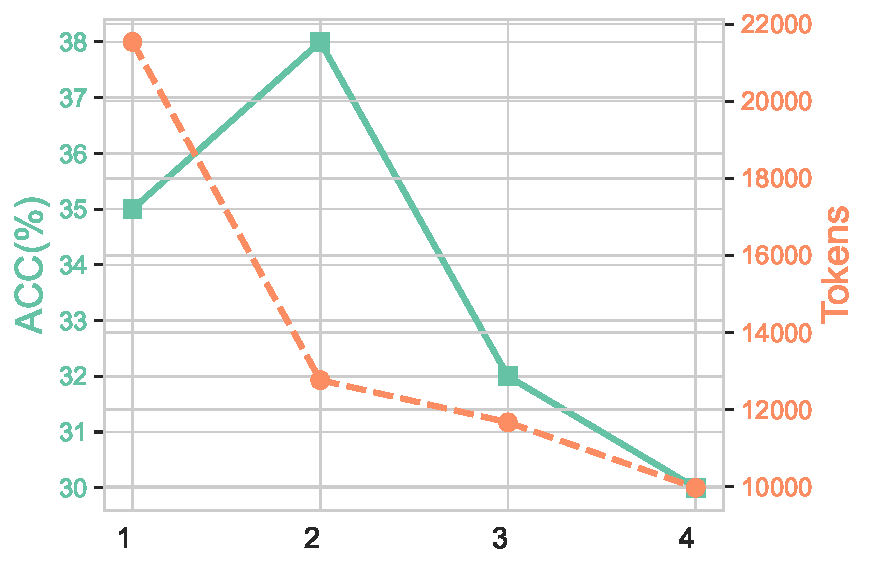
\includegraphics[width=0.8\columnwidth]{figs/intra_group.pdf}
    \caption{\textbf{Different Intra-group Debate Rounds.} The variations in accuracy are brought about by different intra-group rounds $R$.}
    \label{fig8}
\end{figure}

\paragraph{Intra-group Debate Rounds.} To explore the impact of the number of intra-group debate rounds, we conduct analysis under the condition of 4 agents and 4 rounds with varying numbers of intra-group debate rounds. As shown in Figure \ref{fig8}, best accuracy can be achieved when the number of intra-group debate rounds $R$ is 2. This suggests that brief intra-group discussion can achieve better accuracy. Moreover, as $R$ increases, the number of stages $S$ decreases, resulting in lower token cost, which aligns with our derived complexity formula.


\subsection{Scaling Study}
\begin{figure}[t]
    \centering
    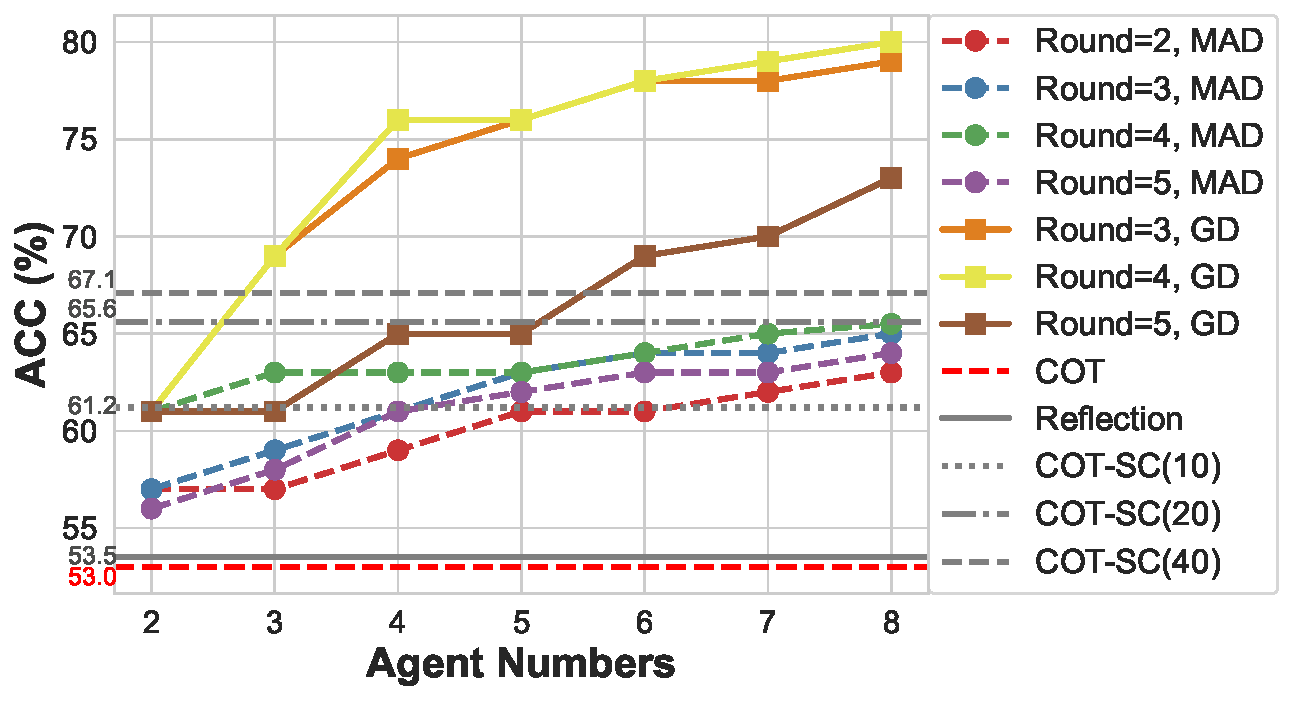
\includegraphics[width=1\columnwidth]{figs/scaling_2.pdf}
    \caption{\textbf{Scaling Study of Agents and Rounds.} }
    \label{fig10}
    % \vspace{-3cm}
\end{figure}

\begin{figure*}
    \centering
    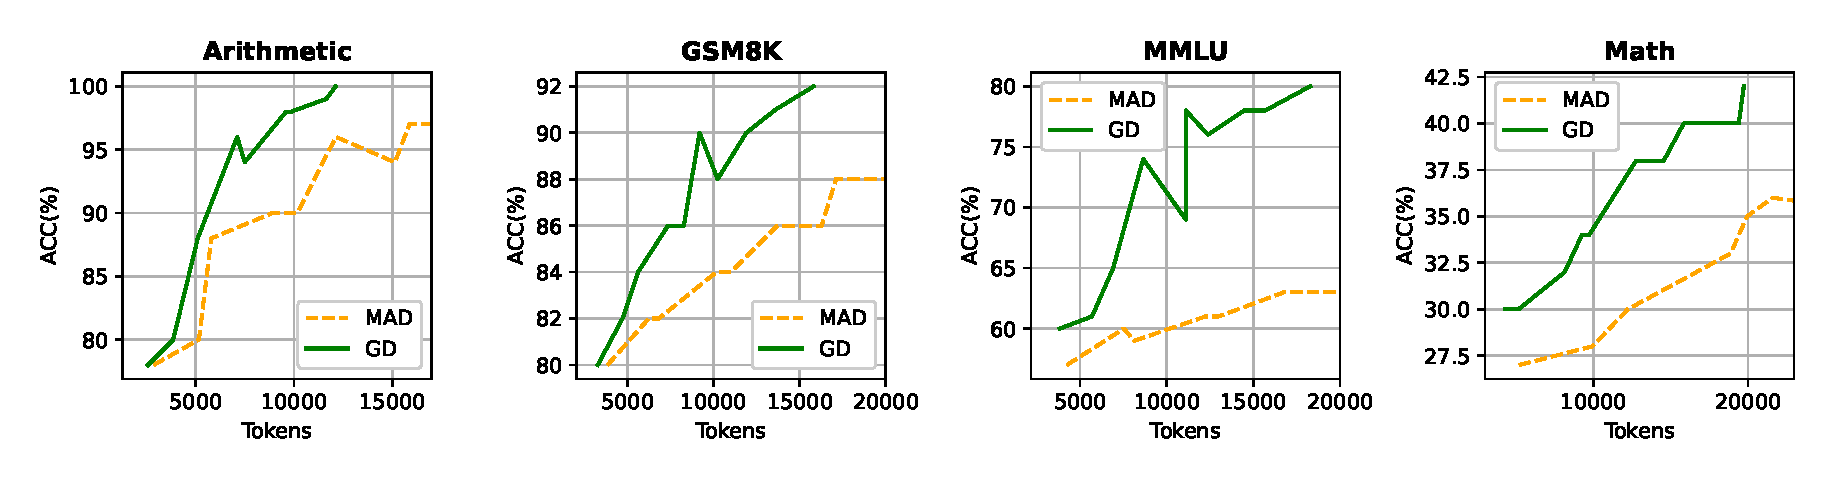
\includegraphics[width=1\linewidth]{figs/scaling_token2.eps}
    \caption{\textbf{Scaling Study of Token Cost.} }
    \label{fig_scaling_token}
\end{figure*}

\paragraph{Agent and Round Scaling.} In order to explore the influence of rounds and agents on accuracy under MAD and GD, we evaluate the changing trends of accuracy for MAD and GD under various rounds and agents. As shown in Figure \ref{fig10}, with the increase in rounds, there is a significant growth in accuracy, but when rounds exceeds 4, a decrease in accuracy is observed across different numbers of agents. This reflects the phenomenon that limited increase in rounds can enhance accuracy, but excessive debate rounds can lead to accuracy degradation. As the number of agents increases, there is a significant growth in accuracy, indicating that an increase in agents can notably enhance the accuracy for both MAD and GD. Concurrently, it should be noted that the rate of improvement in accuracy tends to gradually decelerate as the number of agents continues to rise. The experimental results indicate the importance of controlling the appropriate number of agents and rounds.

\paragraph{Token Scaling.} We assess the scaling trends of token cost and accuracy under both MAD and GD through by increasing the number of rounds or agents. First, as illustrated in Figure \ref{fig_scaling_token}, with the increase in token cost, both MAD and GD exhibit an overall upward trend in accuracy. And initially the accuracy increases rapidly, but as the token cost becomes very large, the rate of accuracy growth slows down. Moreover, GD consistently outperforms MAD with scaling of tokens across all four datasets. While MAD's accuracy tends to converge as the token cost becomes exceedingly large, GD still potentially exhibits a growing trend. And we notice that GD has more sharply increasing points, which may be indicative of emergent intelligence in the token scaling of GD. It's an intriguing research point to explore scaling laws about accuracy and efficiency within multi-agent debate.

\subsection{Ablation Study}
\label{ablation-study}

% \begin{figure*}
%     \centering
%     
\includegraphics[width=0.8\linewidth]{figs/ablation.pdf}
%     \caption{\textbf{Ablation Study.} }
%     \label{fig9}
% \end{figure*}

\begin{figure}[t]
    \centering
    
\includegraphics[width=1\columnwidth]{figs/ablation.pdf}
    \caption{\textbf{Ablation Study.} }
    \label{fig9}
\end{figure}

In order to further investigate the impact of certain components in GD, we conduct a comparative analysis of MAD, MAD+Forget (MAD with only preserving summaries from the previous round), MAD+Group (MAD with group discussion) and GD. First, as illustrated in the Figure \ref{fig9}, GD outperforms all MAD and its variants in token cost and accuracy, which shows the effectiveness of involving both forget mechanism and group discussion in our method. Second, through comparing MAD+Forget with MAD and GD with MAD+Group, the forget mechanism can effectively reduce token cost while maintaining accuracy almost unchanged, which suggests that there is no need for agents to remember all summary results. Third, MAD+Group, compared to MAD+Forget, reduces a substantial number of tokens and significantly improves accuracy. This further highlights the effectiveness of our proposed group discussion method. Based on the grouping strategy analyzed previously, we hypothesize that the primary reason for the enhancement in accuracy is due to the diversity preserved among the groups.